\documentclass[a4paper]{article}

\usepackage[spanish]{babel}
\usepackage{graphicx}
\usepackage{amsmath, amssymb}
\usepackage[margin=2.5cm]{geometry}
\usepackage{fancyhdr}
\usepackage{enumerate}
\usepackage[shortlabels]{enumitem}
\usepackage{parskip}
\usepackage[most]{tcolorbox}
\usepackage[hidelinks]{hyperref}
\usepackage{float}
\usepackage{xcolor}
\usepackage{afterpage}
\usepackage{setspace}

% cabecera
\pagestyle{fancy}
\fancyhead[l]{Semillero de Astronomía}
\fancyhead[c]{Banco de Problemas \#1}
\fancyhead[r]{\today}
\fancyfoot[c]{\thepage}
\renewcommand{\headrulewidth}{0.2pt}

% Comando para espacio vertical
\newcommand{\vsp}{\vspace{0.5cm}}

%% Definicion de comandos para formato de unidades fisicas %%
\newcommand{\m}{\text{m}}
\newcommand{\cm}{\text{cm}}
\newcommand{\km}{\text{km}}
\newcommand{\s}{\text{s}}
\newcommand{\N}{\text{N}}
\newcommand{\g}{\text{g}}
\newcommand{\kg}{\text{kg}}
\newcommand{\Msolar}{\text{M}_\odot}
\newcommand{\Mterrestre}{\text{\text{M}_\oplus}}
\newcommand{\AU}{\text{AU}}
\newcommand{\ly}{\text{ly}}
\newcommand{\nT}{\text{nT}}
\newcommand{\keV}{\text{keV}}
\newcommand{\MeV}{\text{MeV}}
\newcommand{\GeV}{\text{GeV}}
\newcommand{\atoms}{\text{atoms}}
\newcommand{\K}{\text{K}}
\newcommand{\J}{\text{J}}
\newcommand{\particles}{\text{particles}}
\newcommand{\protones}{\text{p}^+}
\newcommand{\electrones}{\text{e}^-}



\begin{document}

% Portada
\begin{titlepage}
    \centering
    
    \vspace*{2cm}
    
    % Título principal - color negro normal
    {\fontsize{36}{40}\selectfont\bfseries BANCO DE PROBLEMAS}
    
    \vsp
    \vsp
    
    % Subtítulo
    {\Large\textbf{Astronomía para las Ciencias Básicas}}
    
    \vsp
    
    {\large Volumen 1}
    
    \vspace{3cm}
    
    \rule{0.7\textwidth}{0.4pt}
    
    \vspace{2.5cm}
    
    {\LARGE\bfseries Institución Educativa}
    
    \vsp
    
    {\LARGE\bfseries Enrique Olaya Herrera}
    
    \vsp
    
    {\LARGE\bfseries (IEEOH)}
    
    \vspace{2.5cm}
    
    {\Large Una iniciativa del:}
    
    \vspace{0.8cm}
    
    \begin{minipage}{0.8\textwidth}
        \centering
        {\fontsize{20}{24}\selectfont\bfseries
        CENTRO DE INTERÉS:}
        
        \vspace{0.4cm}
        
        {\fontsize{24}{28}\selectfont\bfseries
        SEMILLERO DE ASTRONOMÍA}
    \end{minipage}
    
    \vfill
    
    % Espacio para el autor
    \vspace{1.5cm}
    
    \begin{minipage}{\textwidth}
        \centering
        {\large Autor: Daniel Soto} \\
        \vspace{0.3cm}
        {\large \today}
    \end{minipage}
    
    \nopagecolor
    
\end{titlepage}

\section{Fuerza de Marea}

    \begin{figure}[H]
        \centering
        \includegraphics[width=0.7\textwidth]{TidalForce.png}
        \caption{Fuerza de marea entre la tierra y la luna}
        \label{fig:1}
    \end{figure}

  Una fuerza de marea es una diferencia en la intensidad de la gravedad entre dos puntos.
    El campo gravitacional de la luna produce una fuerza de marea a lo largo del diámetro de la Tierra, 
    lo que causa que la Tierra se deforme. También generan mareas de varios metros en la Tierra sólida, 
    y mareas aún más grandes en los océanos líquidos. La Figura \ref{fig:1} muestra una idea de la situación.

    Un ser humano cayendo en un agujero negro también experimentará fuerzas de marea. 
    ¡En la mayoría de los casos estas serán letales! La diferencia en la fuerza gravitacional 
    entre la cabeza y los pies podría ser tan intensa que una persona literalmente sería separada por tracción. 
    Algunos físicos han llamado a este proceso ¡\textit{espaguetificación}! 

    
    \begin{equation}
    a = \frac{2GMd}{R^3}
    \label{eq:1}
    \end{equation}

    \begin{enumerate}
        \item La ecuación \eqref{eq:1} nos permite calcular la aceleración de marea $a$, através de un
        cuerpo de longitud $d$. La aceleración de marea entre tu cabeza y tus pies está dada por la fórmula \ref{eq:1}. 
        Para $M = 5.9\times 10^{27} \text{ g}$ (masa de la tierra), $R=6.4\times 10^8 \text{cm}$ (radio de la tierra) y
        $G=6.67\times 10^{-8} \text{ dyn} \cdot \text{cm}^2/\text{g}^2$, calcula la aceleración de marea, $a$, 
        si una altura humana típica es $d=200\text{ cm}$.
        \item ¿Cuál es la aceleración de marea a través del diámetro completo de la Tierra?
        \item Un agujero negro de masa estelar tiene la masa del sol $(1.9\times 10^{33}\text{ g)}$, 
        y un radio de $2.9 \text{km}$.
        \begin{enumerate}
            \item A una distancia de $100km$, ¿cuál sería la aceleración de marea através de un humano para $d=200cm$
            \item Si la aceleración de gravedad en la superficie de la tierra es $980 	\text{cm/s}^2$, 
            ¿sería espaguetificado el desafortunado viajero humano cerca de un agujero negro de masa estelar?
        \end{enumerate}
        \item Un agujero negro supermasivo tiene $100$ millones de veces la masa del sol, y un radio de $295$ millones de kilómetros.
        ¿Cuál sería la aceleración de marea a través de un humano con $d=2\text{m}$, a una distancia de $100\text{km}$ desde el horizonte 
        de eventos del agujero negro supermasivo?
        \item En qué agujero negro podría entrar un humano sin ser espaguetificado?
    \end{enumerate}

\newpage

\section{Constantes Físicas}

    Aunque solo existen una docena de constantes físicas fundamentales de la naturalez,
    estas se pueden combinar para definir muchas otras constantes básicas en física, 
    química y astronomía.

    \begin{table}[H]
    \centering
    \begin{tabular}{|c|c|c|}
    \hline
    Símbolo & Nombre & Valor \\
    \hline
    $c$ & Velocidad de la Luz & $2.9979\times 10^{10} \text{ cm/s}$\\
    \hline
    $h$ & Constante de Planck & $6.6262\times 10^{-27} \text{ erg}\cdot \text{s}$\\
    \hline
    $m$ & Masa del Electrón & $9.1095\times 10^{-28} \text{ g}$\\
    \hline
    $e$ & Carga del Electrón & $4.80325 \times 10^{-10} \text{esu}$\\
    \hline
    $G$ & Constante de Gravitación & $6.6732 \times 10^{-8} \text{dyn} \cdot \text{cm}^2 \text{gm}^{-2}$\\
    \hline
    $M$ & Masa del Protón & $1.6726 \times 10^{-24} \text{g}$\\
    \hline
    \end{tabular}
    \caption{Constantes físicas}
    \label{tab:3}
    \end{table}
    En este ejercicio, calcularás algunas de estas constantes \textit{secundarias} con una precisión 
    de tres cifras significativas utilizando una calculadora o programación y los valores definidos 
    en la tabla \ref{tab:3}.

    \begin{enumerate}
        \item Constante de entropía de agujero negro $$\frac{c^3}{2hG}$$
        \item Constante de radiación gravitacional $$\frac{32 G^5}{5 c^{10}}$$
        \item Constante de Thomas-Fermi $$\frac{324}{175} \left(\frac{4}{9\pi}\right)^{2/3}$$
        \item Sección transversal de dispersión de Thompson $$\frac{8 \pi}{3} \left(\frac{e^2}{mc^2}\right)^2$$
        \item Límite de Stark $$\frac{1}{M^5} \left(\frac{4 \pi^2 e^2 m}{h^2}\right)^2$$
        \item Constante de radiación de Bremstrahlung $$\frac{32 \pi^2 e^6}{3\sqrt{2\pi}m^3c}$$
        \item Constante de Fotoionización $$\frac{32 \pi^2 e^6 (2\pi^2 e^4 m)}{3^{3/2} h^3}$$
    \end{enumerate}
    
\newpage

\section{Masa Lunar}

El $19$ de Julio de $1969$, el Módulo de Servicio y Comando Apollo-11 y el Módulo Lunar Eagle entraron en órbita lunar.
    \begin{figure}[H]
    \centering
    \includegraphics[width=0.5\textwidth]{moon.png}
    \caption{}
    \label{fig:2}
    \end{figure}
    El tiempo necesario para completar una vuelta completa en la órbita se llama período orbital, 
    que en este caso fue de $2$ horas, a una distancia de $1.737$ km desde el centro de la Luna.

    ¡Crea o no lo creas, puedes usar estas dos piezas de información para determinar la masa de la Luna!
    Así es como se hace:

    \begin{enumerate}
        \item Suponga que el Apollo-11 entró en una órbita circular, y que la aceleración gravitacional hacia
        adentro ejercida por la Luna sobre la cápsula, $F_g/m$, equilibra exactamente la aeleración centrífuga
        hacia afuera, $F_c/m$. Resuelva $F_c=F_g$ para encontrar la masa de la Luna, $M$, en términos de $V$, $R$
        y la constante gravitacional $G$, dado que:
        $$F_g = \frac{GMm}{R^2}\quad\quad F_c = \frac{mV^2}{R}$$
        \item Usando el hecho que para el movimiento circular, $$V = \frac{2\pi R}{T}$$ reexprese su respuesta
        al problema 1 en términos de $R,T$ y $M$.
        \item Dado que $G=6.67\times 10^{-11} \text{ m}^3 \text{kg}^{-1} \text{s}^{-2}$, $R=1.737 \text{ km}$ 
        y $T=2\text{ h}$, calcule la masa de la Luna, $M$, en kilogramos.
        \item La masa de la Tierra es $M = 5.97\times 10^{24} \text{kg}$. ¿Cuál es la razón de la masa de la luna,
        derivada del problema 3, respecto a la pasa de la tierra?
    \end{enumerate}
    
    
\newpage
\section{Temperatura de Equilibrio}

A medida que un cuerpo absorbe energía que incide
    sobre su superficie, también emite enería de vuelta al espacio. 
    Cuando la \textit{energía entrante} iguala a la \textit{energía saliente}, 
    el cuerpo mantiene una temperatura constante de \textit{equilibrio} 

    Si el cuerpo absorbe el $100\%$ de la energía que incide sobre él, 
    la relación entre energía absorbida en $\text{W/m}^2$, $F$, 
    y la temperatura de equilibrio medida en $\text{K}$, $T$, 
    está dada por $$F = 5.7\times 10^{-8} T^4$$
   
    \begin{figure}[H]
        \centering
        \includegraphics[width=0.7\textwidth]{EnceladusTemperatureMap.jpg}
        \caption{Este mapa de temperaturas del satélite Encélado fue creado a partir de los
        datos infrarrojos de la nave espacial Cassini de la NASA}
        \label{fig:3}
    \end{figure}

    \begin{enumerate}
        \item Un cuerpo humano tiene un área superficial de $2\text{ m}^2$ y se encuentra a una 
        temperatura de $98.6\text{ °F}$. 
        ¿Cuál es la potencia total emitida por un ser humano en $\text{W}$?

        \item La luz solar que incide sobre un cuerpo en la Tierra proporciona $1357\text{ W/m}^2$. 
        ¿Cuál sería la temperatura, en $\text{K}$ y $°\text{C}$, del cuerpo si absorbiera 
        completamente todo este flujo de energía solar?

        \item Un flujo de lava de $2000\text{ K}$ tiene $10 \text{ m}$ de ancho y $100\text{ m}$ de largo. 
        ¿Cuál es la potencia térmica total de esta roca caliente en $\text{MW}$

        \item Una pieza de aluminio de $2 \text{ m}^2$ está pintada de modo que absorbe
        solo el $10\%$ de la energía solar que incide sobre ella ($\text{Albedo} = 0.9$). 
        Si el panel de aluminio está en el exterior de la Estación Espacial Internacional, 
        y el flujo solar en el espacio es de $1357\text{ W/m}^2$, 
        ¿Cuál será la temperatura de equilibrio, en $\text{K}$, $\text{°C}$ y $\text{°F}$, del panel bajo plena luz solar?
    \end{enumerate}
    Fórmulas de conversión: $\text{°C}=\text{K}-273$ y $\text{°F}=\frac{9}{5}\text{°C}+32$
    
\newpage
    
\section{Estrellas de Neutrones}

Las estrellas de neutrones son todo lo que queda de una estrella masiva que explotó como una supernova. Propuestas por primera vez hace más de 50 años, estos cuerpos densos, con apenas 50 kilómetros de diámetro, contienen tanta masa como todo nuestro Sol, que apenas tiene 1 millón de kilómetros de diámetro.

    \begin{figure}[H]
        \centering
        \includegraphics[width=0.7\textwidth]{NeutronStar.jpg}
        \caption{Ilustración de una estrella de neutrones en rotación}
        \label{fig:4}
    \end{figure}

Los astrónomos han estudiado docenas de estas estrellas muertas para determinar cuáles pueden ser los rangos de masa de las estrellas de neutrones. Este rango de masa es una pista importante para comprender cómo se ve el interior de estos cuerpos.

Al estudiar los rayos X emitidos por las estrellas de neutrones y al encontrar muchas que están en sistemas binarios de estrellas, se han "pesado" varias estrellas de neutrones. Cinco de ellas han sido medidas detalladamente para componer los siguientes rangos de masa, donde la masa se da en múltiplos de masas solares ($\text{M}_{\odot} = 2\times 10^{30}\text{ kg}$):

	\begin{table}[H]
   		\centering
        \begin{tabular}{|c|c|}
        	\hline
        	Fuente de emisión de rayos X & Rango de masa [$\text{M}_{\odot}$] \\
            \hline
            3U0900-40 & $1.2 < M < 2.4$ \\
            \hline    
            Centaurus X-3 & $0.7 < M < 4.3$ \\
            \hline
            SMC X-1 & $0.8 < M < 1.8$ \\
            \hline
            Hercules X-1 & $0.0 < M < 2.3$ \\
            \hline
        \end{tabular}
        \caption{Rangos de masa estimados para cinco estrellas de neutrones detectadas mediante su emisión de rayos X en sistemas binarios}
        \label{tab:1}
    \end{table}

    \begin{enumerate}
    	\item ¿Cuál es el punto de intersección de estos límites para las masas de las estrellas de neutrones?
        \item ¿Cuál es el rango de masa permitido para una estrella de neutrones en kilogramos?
    \end{enumerate}


\newpage

\section{Poder de Resolución del Telescopio}

El tamaño de un espejo de telescopio determina qué tan bien puede resolver detalles en objetos distantes.

    \begin{figure}[H]
        \centering
        \includegraphics[width=0.7\textwidth]{MirrorHubble.jpg}
		\caption{Espejo del telescopio espacial Hubble en 1993}
        \label{fig:5}
    \end{figure}
     
Los astrónomos siempre están construyendo telescopios más grandes para ayudarles a ver el universo lejano con mayor claridad.
	\begin{enumerate}
		\item Esta sencilla función predice la resolución $R(D)$,  en segundos de arco ($\text{''}$), de un espejo de telescopio cuyo diámetro, 
		$D$, se da en centímetros:
		
		$$R(D) = \frac{10.3}{D} \text{ ''}$$
		
		Si el dominio de $R(D)$ abarca desde el tamaño de un ojo humano ($0.5\text{ cm}$) hasta el diámetro del Telescopio Espacial Hubble
		 ($240 \text{ cm}$),¿Cuál es el rango angular de $R(D)$ en segundos de arco?
		\item Complete los números faltantes en la forma tabular de $R(D)$ que se muestra a continuación.
		\begin{table}[H]
		     \centering
		     \begin{tabular}{|c|c|c|c|c|c|c|c|c|c|c|}
		         \hline
		         D & & 1 & & 20 & & 100 & & 200 & \\ 
		         \hline
		         R(D) & 21.0 & & 2.1 & & 0.21 & & 0.069 & & 0.043 \\
		         \hline
		     \end{tabular}
		     \caption{Valores de la función $R(D)$ para diferentes diámetros $D$.}
		     \label{tab:2}
		 \end{table} 
		Utilice una precisión de dos cifras significativas, redondeando cuando sea apropiado.
	\end{enumerate}

\newpage
\section{Cúmulos Estelares}
 \begin{figure}[H]
        \centering
        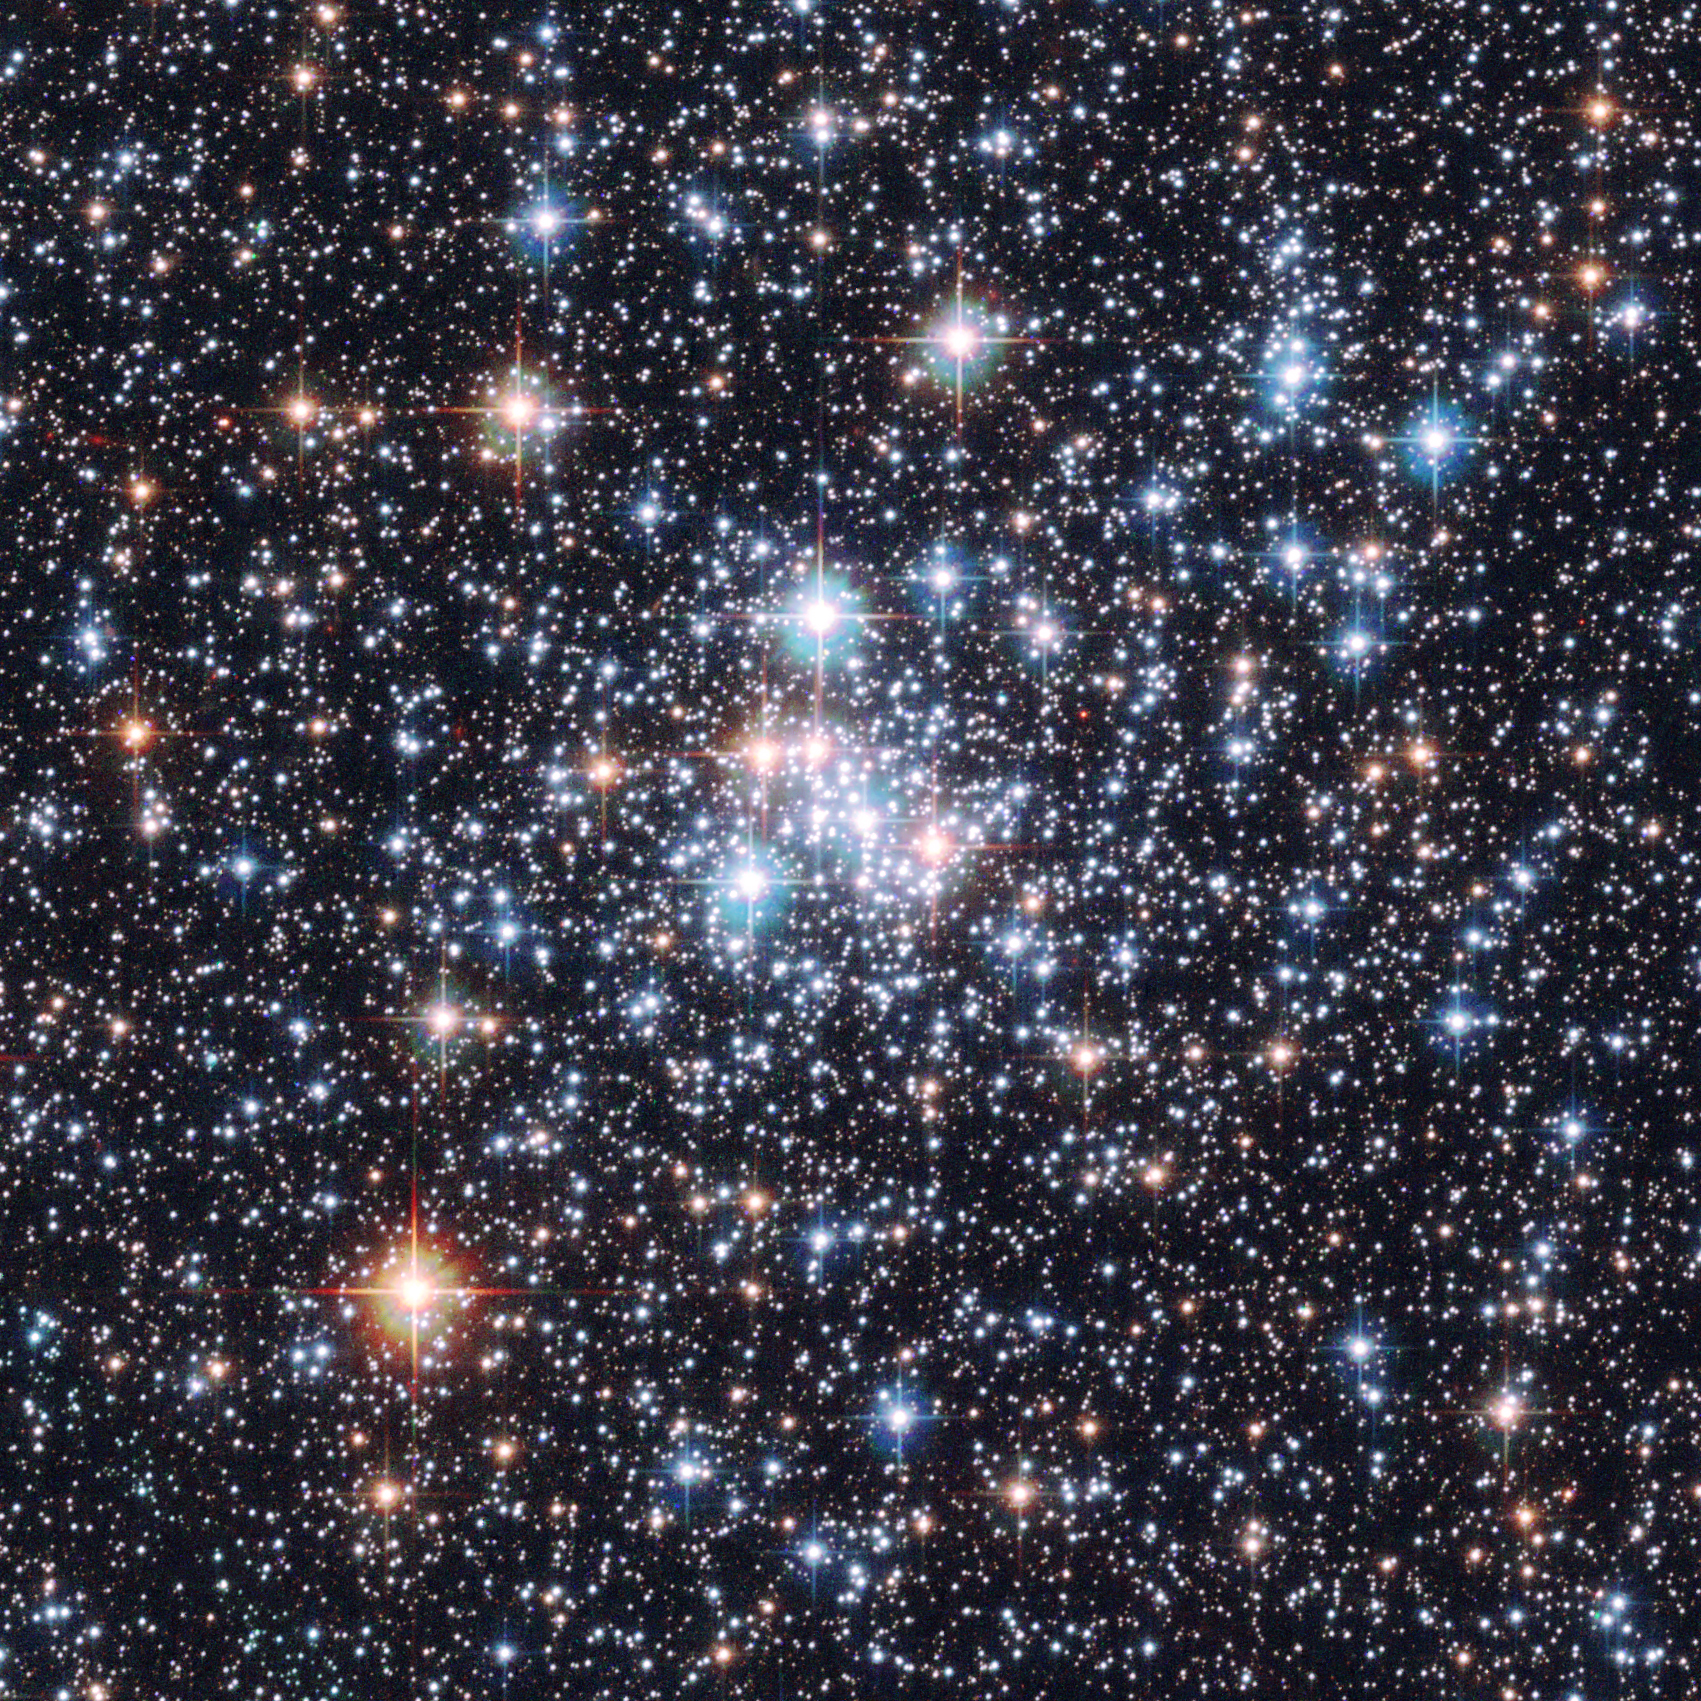
\includegraphics[width=0.5\textwidth]{StarCluster.jpg}
        \caption{Telescopio espacial Hubble: Cúmulo Estelar NGC 290}
        \label{fig:6}
    \end{figure}
  Como se muestra en la Figura \ref{fig:6}, consisten en cientos de estrellas que se mueven por el 
    espacio como una sola unidad.
    
    Los astrónomos necesitan conocer las masas de estos cúmulos, junto con la cantidad los diferentes tipos de estrellas que 
    los componen, para estudiar cómo se forman y cambian los cúmulos estelares con el tiempo.
    
    El cúmulo estelar NGC-290, mostrado en la foto del Telescopio Espacial Hubble, se encuentra en la galaxia cercana llamada 
    Nube Menor de Magallanes, a unos 200000 años luz de la Tierra.
    
    Los astrónomos utilizan la masa de nuestro Sol como una unidad conveniente de masas al comparar otras estrellas 
    ¡1 masa solar $[M_\odot]$ equivale a aproximadamente 2000 billones de toneladas! 
    \vspace{5mm}
	\begin{enumerate}
		\item Supongamos que NGC-290 tiene una masa total de no más de 500 $M_\odot$. 
		Si está compuesto por estrellas azules gigantes luminosas de tipo B con masas individuales de 10 $M_\odot$, 
		y estrellas rojas supergigantes antiguas de tipo M con masas individuales de 30 $M_\odot$, grafique una desigualdad 
		que muestre el número de estrellas B y M en este cúmulo. Escriba una desigualdad que represente esta información 
		y resuélvala gráficamente.
	
	    \item ¿La combinación de 9 estrellas de tipo B y 32 estrellas de tipo M conduce a una solución de población posible para este cúmulo?
	\end{enumerate}
	
\newpage
\section{Èpocas del Universo}
El universo ha pasado por tres etapas diferentes de expansión poco después de Big Bang. 
	Los astrónomos llaman a estas etapas: \textit{Era Inflacionaria}, \textit{Era de Radiación} y \textit{Era de Materia}.
	
	\begin{figure}[H]
	        \centering
	        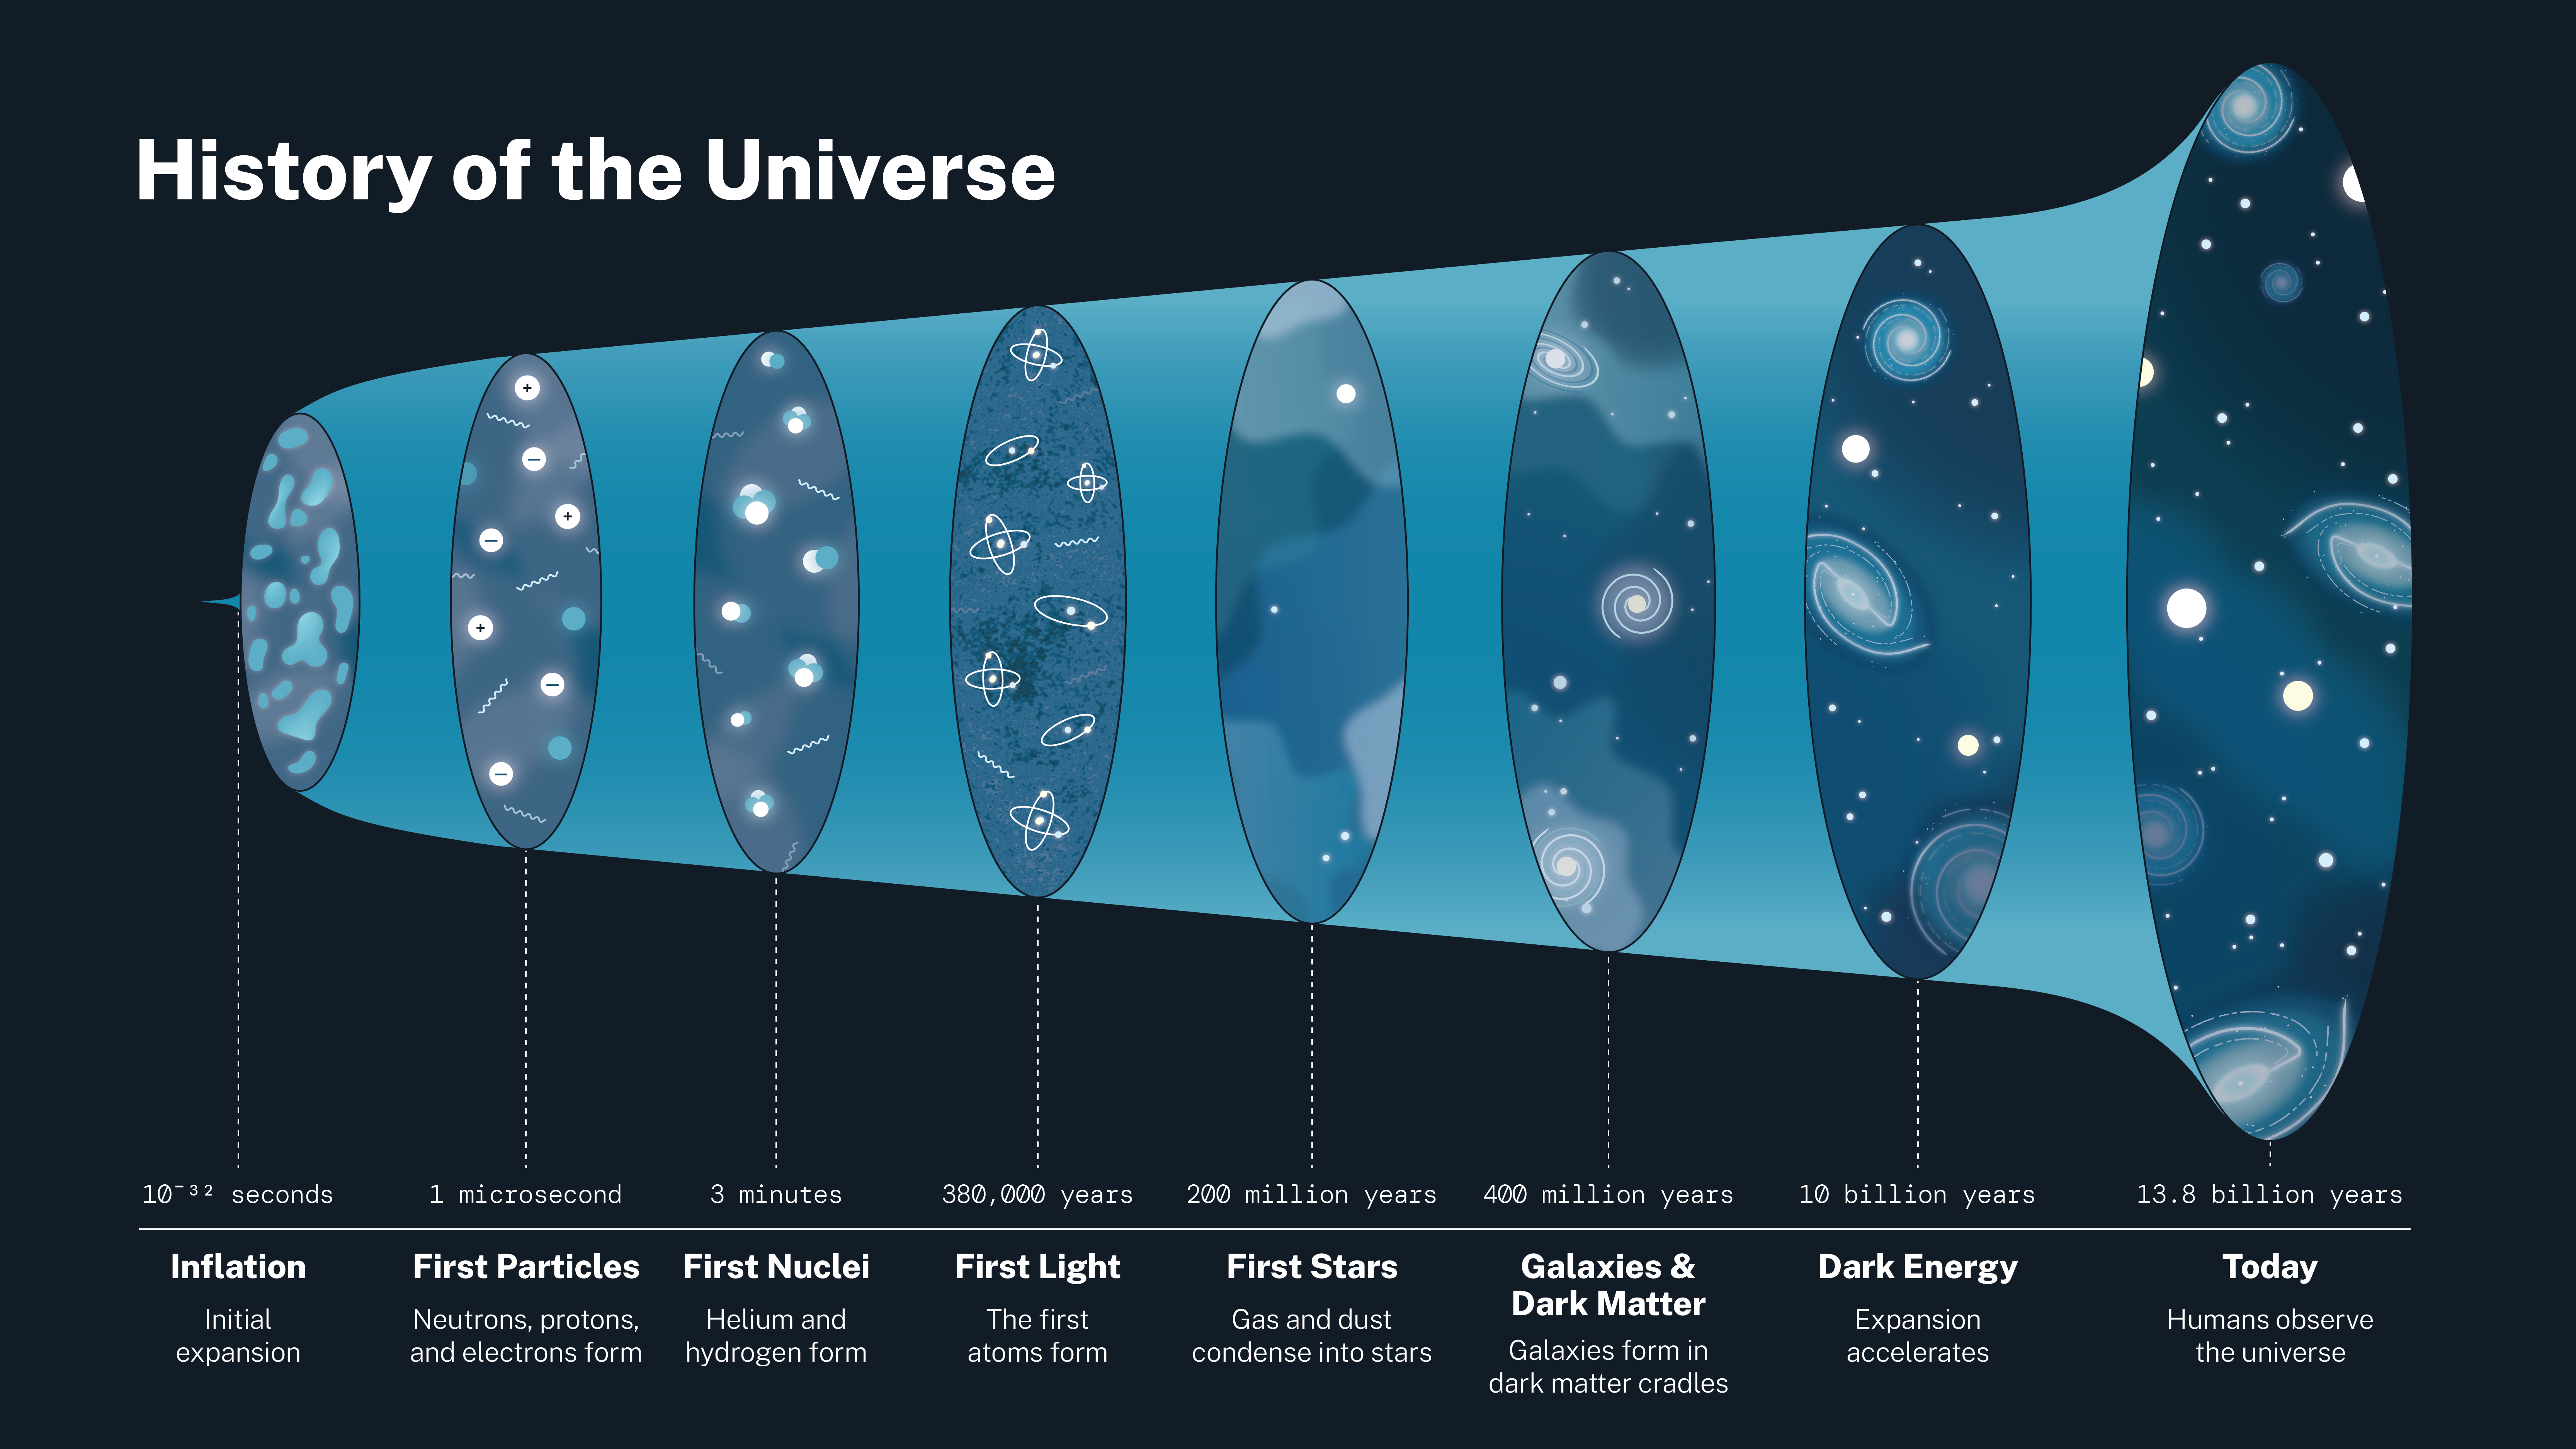
\includegraphics[width=\textwidth]{CosmicEpochs.png}
	        \caption{Diferentes épocas cósmicas}
	        \label{fig:7}
	\end{figure}
	El tamaño del universo está determinado por las separaciones entre objetos típicos, y puede representarse 
	mediante modelos matemáticos basados en las ecuaciones físicas que rigen el comportamiento de la materia, 
	la energía y la gravedad.
	
	La expansión del universo puede definirse mediante la siguiente función definida a trozos, donde la variable $t$ 
	se mide en segundos desde el Big Bang:
	
	$$ a(t) = \left\{\begin{matrix}
	2.2\times 10^{-29}e^{10^{35t}} & 10^{-35} < t < 10^{-33} \quad\text{Era de Inflación} \\
	6.4\times 10^{10}\sqrt{t} & 10^{-33} < t < 9.3\times 10^{12} \quad\text{Era de Radiación} \\
	7700 t ^ {4/3} & 9.3\times 10^{12} < t < 4.2\times 10^{17} \quad\text{Era de la Materia}
	\end{matrix}\right.$$
	\vspace{5mm}
	\begin{enumerate}
		\item ¿Cuál es la gráfica de $a(t)$ entre 1 segundo y 10 minutos después del Big Bang?
	
		\item ¿Cuál es la gráfica de $a(t)$ entre 12 y 13 mil millones de años después del Big Bang?
	
		\item ¿En qué factor cambia $a(t)$ cuando el tiempo trancurrido desde el Big Bang aumenta en un factor de 10 durante cada era?
	\end{enumerate}

\newpage
\section{Movimiento vertical bajo gravedad}
\begin{figure}[H]
	        \centering
	        \includegraphics[width=\textwidth]{VerticalMotionGravity.jpeg}
	        \caption{Marte, Luna y Tierra}
	        \label{fig:8}
	\end{figure}

	\textbf{Movimiento vertical bajo la gravedad:} La expresión común 'lo que sube, debe bajar' puede representarse mediante 
	una ecuación cuadrática. Si trazara la altura de una pelota lanzada verticalmente, su altura en función del tiempo seguiría 
	una sencilla fórmula cuadrática dada por la ecuación general:

	$$H(t) = h_0 +vt - \frac{1}{2}g t^2$$

	donde $h_0$ es la altura inicial de la pelota en metros, $v$ es la velocidad inicial en $\text{m/s}$, y $g$ es la 
	aceleración de la gravedad en $\text{m/s}^2$. Es una ecuación general porque funciona no solo en la Tierra, 
	sino también en casi todos los demás cuerpos astronómicos, excepto en los agujeros negros. Para los agujeros negros, 
	la geometría del espacio está tan distorsionada que $t, v$ y $h_0$ se alteran de formas complejas.

	\vspace{5mm}

	Para los siguientes problemas:

	\vspace{5mm}

	\begin{itemize}
		\item Escriba la ecuación en forma estándar.

		\item Determine las coordenadas del vértice de la parábola donde $H(t)$ es máximo.

		\item Determine el eje de simetría.

		\item En una misma gráfica para los tres problemas, trace la parábola para cada problema 
		graficando dos puntos adicionales utilizando la propiedad del eje de simetría, para todos los 
		tiempos positivos durante los cuales $H(t)>0$
	\end{itemize}
	
	\vspace{5mm}

	\begin{enumerate}
		\item En la Tierra, la aceleración de la gravedad es $g=10 \text{ m/s}^2$. 
		La pelota fue lanzada verticalmente hacia arriba con una velocidad inicial 
		de $v=20\text{ m/s}$ desde una altura de $h_0=2\text{ m}$.
	
		\item En Marte, la aceleración de la gravedad es $g=4 \text{ m/s}^2$. 
		La pelota fue lanzada verticalmente hacia arriba con una velocidad inicial 
		de $v=20\text{ m/s}$ desde una altura de $h_0=2\text{ m}$.

		\item En la Luna, la aceleración de la gravedad es $g=2 \text{ m/s}^2$. 
		La pelota fue lanzada verticalmente hacia arriba con una velocidad inicial 
		de $v=20\text{ m/s}$ desde una altura de $h_0=2\text{ m}$.
	\end{enumerate}


\newpage
\section{Energía potencial y cinética}
La energía potencial es la energía que posee un cuerpo debido a su ubicación en el espacio, mientras que la energía cinética es la que depende de su velocidad en el espacio. Para ubicaciones dentro de los cuatrocientos kilómetros de la superficie terrestre, despreciando la resistencia del aire y para velocidades que son pequeñas en comparación con la de la luz, tenemos las siguientes fórmulas de energía.

$$E_P = mgh\quad\quad E_k = \frac{1}{2}mv^2$$

donde $g$ es la aceleración de la gravedad cerca de la superficie terrestre y tiene un valor de $9.8 \m/\s^2$. Si utilizamos las unidades de masa, $m$, en $\kg$, altura sobre el suelo, h, en $\m$, y la velocidad del cuerpo, $v$, en $\m/\s$, las unidades de energía son $\J$ (Joules).

    \begin{figure}[H]
        \centering
        \includegraphics[width=0.7\textwidth]{Ares1x.jpg}
        \caption{Cohete Ares 1-X}
        \label{fig:9}
    \end{figure}

Al igual que una pelota de béisbol, un cohete en caída libre o una piedra lanzada desde un puente se mueven a lo largo de su trayectoria hacia el suelo. Constantemente intercambian joules de energía potencial por energía cinética. Antes de caer, su energía es $100\%$ $E_p$, mientras que en el instante justo antes de tocar tierra, su energía es $100\%$ $E_k$.
\begin{enumerate}
	\item Una pelota de béisbol con $m = 0.145 \kg$ cae desde la parte superior de su arco hasta el suelo, a una distancia de $100 \m$.
		\begin{enumerate}
		\item ¿Cuál era su $E_k$ en $\text{J}$, en la parte superior de su arco?
		\item ¿Cuál era la $E_p$ de la pelota de béisbol, en $\J$, en la parte superior de su arco?
		\end{enumerate}
	\item La cápsula Ares 1-X tenía una masa de 5000 $\kg$. Si la cápsula cayó $45\km$ desde la parte superior de su trayectoria, ¿Cuánta energía cinética tenía en el momento del impacto con el suelo?
	\item Suponga que la pelota de béisbol del \textit{Problema 1} se dejó caer desde la misma altura que la cápsula Ares 1-X. ¿Cuál sería su $E_k$ en el momento del impacto?
	\item A partir de la fórmula para $E_k$ y sus respuestas a \textit{los problemas 2 y 3}, en $\m/\s$:
		\begin{enumerate}
		\item ¿Cuál fue la velocidad de la pelota de béisbol cuando golpeó el suelo?
		\item ¿Cuál fue la velocidad de la cápsula Ares 1-X cuando aterrizó?
		\item Discuta por qué sus respuestas no parecen tener sentido.
		\end{enumerate}
\end{enumerate}


\newpage
\section{Tamaños en el Universo}

El universo es un lugar MUY grande... ¡Pero también tiene algunos ingredientes muy pequeños! Los astrónomos y físicos a menudo encuentran que las escalas lineales para graficar son muy incómodas de usar porque las cantidades que más les gustaría graficar difieren en potencias de $10$ en tamaño, temperatura o masa. Las gráficas \textit{Log-Log} se utilizan comúnmente para ver la \textit{imagen general}. En lugar de una escala lineal como $1\km, 2\km, 3\km, ...,$ se utiliza una escala logarítmica donde $1$ representa $10^1$, $2$ representa $10^2$, ..., $20$ representa $10^{20}$, etc.

\begin{table}[H]
\centering
\begin{tabular}{|c|c|c|c|}
\hline
\# & Objeto & R (metros) & M (kg) \\
\hline
1 & Tú & $2.0$ & $60$ \\
\hline
2 & Mosquito & $2 \times 10^{-3}$ & $2 \times 10^{-6}$ \\
\hline
3 & Protón & $2 \times 10^{-15}$ & $2 \times 10^{-27}$ \\
\hline
4 & Electrón & $4 \times 10^{-18}$ & $1 \times 10^{-30}$ \\
\hline
5 & Bosón Z & $1 \times 10^{-18}$ & $2 \times 10^{-25}$ \\
\hline
6 & Tierra & $6 \times 10^{6}$ & $6 \times 10^{24}$ \\
\hline
7 & Sol & $1 \times 10^{9}$ & $2 \times 10^{30}$ \\
\hline
8 & Júpiter & $4 \times 10^{8}$ & $2 \times 10^{27}$ \\
\hline
9 & Betelgeuse & $8 \times 10^{11}$ & $6 \times 10^{31}$ \\
\hline
10 & Galaxia Vía Láctea & $1 \times 10^{21}$ & $5 \times 10^{41}$ \\
\hline
11 & Átomo de uranio & $2 \times 10^{-14}$ & $4 \times 10^{-25}$ \\
\hline
12 & Sistema solar & $1 \times 10^{13}$ & $2 \times 10^{30}$ \\
\hline
13 & Ameba & $6 \times 10^{-5}$ & $1 \times 10^{-12}$ \\
\hline
14 & Bombilla de 100 vatios & $5 \times 10^{-2}$ & $5 \times 10^{-2}$ \\
\hline
15 & Enana blanca Sirius B & $6 \times 10^{6}$ & $2 \times 10^{30}$ \\
\hline
16 & Nebulosa de Orión & $3 \times 10^{18}$ & $2 \times 10^{34}$ \\
\hline
17 & Estrella de neutrones & $4 \times 10^{4}$ & $4 \times 10^{30}$ \\
\hline
18 & Sistema binario de estrellas & $1 \times 10^{13}$ & $4 \times 10^{30}$ \\
\hline
19 & Cúmulo globular M13 & $1 \times 10^{18}$ & $2 \times 10^{35}$ \\
\hline
20 & Cúmulo de galaxias & $5 \times 10^{23}$ & $5 \times 10^{44}$ \\
\hline
21 & Universo visible & $2 \times 10^{26}$ & $2 \times 10^{54}$ \\
\hline
\end{tabular}
\caption{Objetos, sus radios y masas típicos}
\label{tab:objetos}
\end{table}

A continuación trabajaremos con una gráfica $\log(m)$ vs $\log(r)$, donde $m$ es la masa de un objeto en kilogramos y $r$ es su longitud o diámetro en metros.
\begin{enumerate}
	\item Grafica los objetos enumerados en la tabla a continuación en una gráfica \textit{Log-Log}, con el eje $x$ siendo $\log(M)$ y el eje $y$ siendo $\log(r)$.

	\item Dibuja una línea que represente todos los objetos que tienen una densidad de
	\begin{enumerate} 
		\item$N\to$ materia nuclear: $4 \times 10^{17} \km/\m^3$
		\item $W\to$ agua: $1000 \km/\m^3$.
	\end{enumerate}
	\item Los agujeros negros se definen mediante la sencilla fórmula $R = 3M$, donde $R$ es el radio en kilómetros y $M$ es la masa en unidades de masas solares ($M_\odot = 2 \times 10^{30} \kg$). Sombrea la región de la 		gráfica \textit{Log-Log} que representa la condición de que ningún objeto de una masa dada puede tener un radio \textbf{menor} que el de un agujero negro.

	\item La densidad más baja alcanzable en nuestro universo está determinada por la densidad del campo de radiación del fuego cósmico, de $4 \times 10^{-31} \kg/\m^3$. Dibuja una línea que identifique el lugar geométrico de 			los objetos con esta densidad, y sombrea la región que excluye densidades \textbf{menores} que esta.
\end{enumerate}


\newpage
\section{Ciclo de Manchas Solares}

    \begin{figure}[H]
        \centering
        \includegraphics[width=0.7\textwidth]{SunspotCycle.png}
        \caption{Ciclo de manchas solares}
        \label{fig:10}
    \end{figure}
    
Las manchas solares aparecen y desaparecen en un ciclo de aproximadamente 11 años. Los astrónomos miden la simetría de estos ciclos comparando los primeros 4 años con los últimos 4 años. Si los ciclos son exactamente simétricos, las diferencias correspondientes serán exactamente cero.

\begin{table}[H]
\centering
\begin{tabular}{|c|c|c|c|c|}
\hline
\textbf{Matriz A} & \textbf{Año 1} & \textbf{Año 2} & \textbf{Año 3} & \textbf{Año 4} \\
\hline
Ciclo 23 & 21 & 64 & 93 & 119 \\
\hline
Ciclo 22 & 13 & 29 & 100 & 157 \\
\hline
Ciclo 21 & 12 & 27 & 92 & 155 \\
\hline
Ciclo 20 & 15 & 47 & 93 & 106 \\
\hline
\end{tabular}
\caption{Número de manchas solares al inicio de cada ciclo}
\label{tab:matrizA}
\end{table}

\begin{table}[H]
\centering
\begin{tabular}{|c|c|c|c|c|}
\hline
\textbf{Matriz B} & \textbf{Año 11} & \textbf{Año 10} & \textbf{Año 9} & \textbf{Año 8} \\
\hline
Ciclo 23 & 8 & 15 & 29 & 40 \\
\hline
Ciclo 22 & 8 & 17 & 30 & 54 \\
\hline
Ciclo 21 & 15 & 34 & 38 & 64 \\
\hline
Ciclo 20 & 10 & 28 & 38 & 54 \\
\hline
\end{tabular}
\caption{Número de manchas solares al final de cada ciclo}
\label{tab:matrizB}
\end{table}

\begin{enumerate}
	\item Calcula el promedio de los números de manchas solares para cada ciclo según $C = \frac{A+B}{2}$
	\item Calcula la diferencia promedio de los números de manchas solares entre el inicio y el final de cada ciclo según $D = \frac{A-B}{2}$
	\item ¿Son simétricos los ciclos?
\end{enumerate}

\newpage

    
\cite{algebra2}
\bibliographystyle{plainurl}
\bibliography{bibliografia} % Nombre del .bib
\end{document}